\documentclass[11pt,letterpaper]{article}

\usepackage{textcomp,marvosym}
\usepackage{amsmath,amssymb}
\usepackage[left]{lineno}
\usepackage{changepage}
\usepackage{rotating}
\usepackage{natbib}
\usepackage{setspace}
\usepackage{fancyhdr}
\usepackage{graphicx}
\usepackage[aboveskip=1pt,labelfont=bf,labelsep=period,justification=raggedright,singlelinecheck=off]{caption}
\doublespacing

\raggedright
\textwidth = 6.5 in
\textheight = 8.25 in
\oddsidemargin = 0.0 in
\evensidemargin = 0.0 in
\topmargin = 0.0 in
\headheight = 0.0 in
\headsep = 0.5 in
\parskip = 0.1 in
\parindent = 0.2in

\pagestyle{myheadings}
\pagestyle{fancy}
\fancyhf{}
\lhead{Swanson-Hysell et al., to be submitted to GEOLOGY}
\rhead{\thepage}

\begin{document}

\begin{flushleft}
{\Large \textbf{Primary red bed magnetization revealed by fluvial intraclasts}}
\\
Nicholas L. Swanson-Hysell\textsuperscript{1},
Luke M. Fairchild\textsuperscript{1},
Sarah P. Slotznick\textsuperscript{1}
\\
\bigskip
\textsuperscript{1} Department of Earth and Planetary Science, University of California, Berkeley, CA, USA
\bigskip

\end{flushleft}

\noindent\textit{This article is to be submitted for consideration at GEOLOGY (published by the Geological Society of America).}

\linenumbers
\pagestyle{empty}

\section*{ABSTRACT}

The magnetization of hematite-bearing sedimentary rocks provides critical records of geomagnetic reversals and paleogeography. However, the timing of acquisition of remanent magnetization held by hematite is typically difficult to constrain and has led to much controversy in the interpretation of such data. This so-called ``red bed controversy'' stems from the reality that while detrital hematite in sediment can lead to a primary depositional remanent magnetization, alteration of minerals through interaction with oxygenated fluids in the near-surface environment can lead to the formation of hematite following deposition. Growth of hematite crystals within sediments could occur in a geologically short time period in the near-surface immediately following deposition or could occur thousands to millions of years later due to the passage of oxygenated fluids following burial. Given that many paleomagnetic field tests such as the reversal test and fold test could still ``pass'' in scenarios with post-depositional secondary hematite growth, this problem has been particularly intractable in many successions. In this study, we use an exceptionally well-preserved ancient fluvial deposit within the 1.1 billion year old Freda Formation to gain insight into the timing of hematite remanence acquisition. This deposit contains siltstone intraclasts, from a coexisting lithofacies of fine-grained over-bank deposits, that were redeposited into channel sandstone. Thermal demagnetization and petrographic data from these clasts reveal that they contain two generations of hematite. One population of hematite was removed at the highest unblocking temperatures and records directions that were rotated when the rip-up clasts were liberated and redeposited. This component is therefore interpreted as a primary detrital remanent magnetization that formed prior to the reorientation of the clasts within the river. The other component is removed at lower unblocking temperatures and has a consistent direction throughout the intraclasts. This component is held by a population of finer-grained hematite that acquired a chemical remanent magnetization as it formed following deposition. The context of these samples enable the complexity of these two generations of hematite to be revealed. The data support the interpretation that the magnetization of hematite-bearing sedimentary rocks held by $>$400 $mu$m is more likely to record magnetization from the time of deposition and can be successfully isolated from co-occurring authigenic hematite.

\section*{INTRODUCTION}

The magnetizations of hematite-bearing sedimentary rocks known as ``red beds'' have provided ample opportunities for Earth scientists to gain insight into the ancient geomagnetic field and the past positions of sedimentary basins. However, with these opportunities has come much consternation leading to what has been referred to as the ``red bed controversy'' \citep{Butler1992a, Beck2003b, Van-Der-Voo2012a}. This controversy stems from the reality that hematite within sedimentary rocks can have two sources: 1) as detrital grains that are delivered to the sediment at the time of deposition and 2) as grains that grow insitu after the sediments have been deposited.

How does one constrain the timing of the acquisition of hematite in sedimentary rocks? Many of the traditional paleomagnetic field tests are unable to differentiate between primary versus diagenetic remanence. For example, a structural fold test can constrain that a remanence direction was obtained prior to structural tilting, but millions of years have typically passed between the deposition of a sediment, its burial in a sedimentary basin and such tectonic tilting. Dual polarity directions through a sedimentary succession are commonly interpreted as providing assurance that the remanence records primary or near-primary magnetization, but it is possible that hematite growth occurred at a time significantly after deposition during a period when the geomagnetic field was reversing. Petrographic investigation of the sedimentary rocks of interest are valuable, but it can be difficult to ascertain the overall contribution to the magnetization of hematite that is petrographically observed and to unambiguously interpret whether an observed grain is in fact detrital (e.g. \citealp{Elmore1982a}). A common grouping of grains within hematite-rich sediment is to consider that there is a fine-grained pigmentary population that formed within the sediment and a coarser-grained population that has been referred to in the literature as ``specularite'' \citep{Butler1992a, Van-Der-Voo2012a}. The work of \cite{Tauxe1980a} showed that sediments with abundant red pigmentary hematite in the Miocene Siwalik Group had lower thermal unblocking temperatures than grey samples dominated by a coarser-grained phase of specular hematite. Observations such as these have led to the practice of defining the characteristic remanent magnetization from hematite bearing sediments as that held by the highest unblocking temperatures \citep{Van-Der-Voo2012a}.  The primary versus secondary nature of micron-scale ``specularite'' grains that likely carry this remanence has been one of the largest sources of contention in the ``red bed controversy'' \citep{Van-Houten1968a, Tauxe1980a, Butler1992a, Van-Der-Voo2012a}.

What is needed to address the timing of remanence acquisition is a process that reorients the sediment before it has been lithified. Two such processes that can occur within a siliciclastic depositional environment and be preserved in the rock record are: 1) syn-sedimentary slumping wherein coherent sediment is reoriented through soft-sediment folding in the surface environment and 2) intraclasts comprised of the lithology of interest that have been liberated and redeposited within the depositional environment. In sediments that have undergone these sedimentary processes that have caused reorientation, significant insight can be gained as to whether magnetization was acquired before or after reorientation. 

\cite{Tauxe1980a} studied 7 cobble-sized clasts within the Siwalik Group that were interpreted to have formed by cut bank collapse and discovered that their magnetic remanence was acquired prior to clast reorientation. An investigation by \cite{Purucker1980a} on red beds of the Triassic Moenkopi Formation of Arizona used multiple such processes to gain insight into hematite acquisition. In their study, an intraformational landslide deposit with isoclinal folds of hematite-bearing claystone revealed non-uniform directions upon blanket demagnetization to 650\textdegree C that cluster better when corrected for their tilt. Scatter was also observed in intraformational conglomerate clasts weathered out of an underlying unit upon blanket thermal demagnetization to 630\textdegree C, but the lack of principal component analysis makes it difficult to evaluate the coherency of the directions. This limitation is found in many studies from this era of research when the red bed controversy was particularly fervent as the work predates the widespread application of principal component analysis in conjunction with systematic progressive thermal demagnetization \citep{Kirschvink1980a, Van-Der-Voo2012a}. For example, \cite{Larson1982b} analyzed shale rip-up clasts in the same Moenkopi Formation and used the fact that similar remanence directions were removed between clasts during low-resolution thermal demagnetization up to 645\textdegree C to support their preferred hypothesis that red beds rarely reflect the geomagnetic field at the time of deposition. However, the cessation of thermal demagnetization well below the N\'eel temperature of hematite in this analysis and the lack of principal component analysis makes it difficult to evaluate this conclusion.  

In this study, we investigate cm-scale siltstone intraclasts within the Freda Formation that were eroded by fluvial processes and redeposited amongst cross-stratified sandstones (Fig. \ref{fig:intraclast_images}). High-resolution thermal demagnetization data on these clasts provide constrain the timing of hematite acquisition by revealing a primary component that formed prior to the liberation of the clasts and a secondary component that formed following their redeposition.

\section*{GEOLOGICAL SETTING}

The $\sim$4 km thick Freda Formation was deposited in the Midcontinent Rift contemporaneous with the final record of regional volcanism and during the subsequent time period when the region was thermally subsiding \citep{Cannon1992a}. The fluvial sediments of the Freda Formation are part of the Oronto Group and were deposited following the deposition of the alluvial Copper Harbor Conglomerate and the lacustrine Nonesuch Formation \citep{Ojakangas2001a}. The underlying Copper Harbor Conglomerate has lava flows within it on the Keweenaw Peninsula and one of these flows has an U-Pb date of 1085.57 $\pm$ 0.25/1.3 Ma (2$\sigma$ analytical/analytical+tracer+decay constant uncertainty; \citealp{Fairchild2017a}). Abundant fine-grained red siltstones within the formation have a well-behaved magnetic remanence dominated by hematite \citep{Henry1977a}.

\begin{figure}[!ht]
\centering
\noindent\includegraphics[width=0.9\textwidth]{BRIC_clast_images.png}
\caption{\small{A: Siltstone intraclasts within the Freda Formation. The field photo shows an intact layer of siltstone below the hammer head which is topped by a bed of trough cross-stratified coarse sandstone with horizons of siltstone intraclasts. The hammer is 40 cm long. Some of the intraclasts are pointed to with arrows. The close-up inset photo is of an individual intraclast that was sampled as BRIC.26. B: A scan of a 30 $\mu$m-thick thin section of the BRIC.26 intraclast (upper half of image) and the coarse sand matrix (lower half of image). The red color of the intraclast is due to the pigmentary hematite. C: Scanning electron microscopy backscattered image of the siltstone clast. The light-colored detrital grains (light due to higher atomic number than the silicate grains) labeled with arrows were confirmed to be hematite through electron backscatter diffraction.}}
\label{fig:intraclast_images}
\end{figure} 

The studied exposure outcrops along the Bad River in northern Wisconsin in the lower portion of the Freda Formation approximately 400 meters above its conformable base with the underlying Nonesuch Formation.\footnote{GSA Data Repository item 2018XXX, is available online at www.geosociety.org/pubs/ft2018.htm, or on request from editing@geosociety.org or Documents Secretary, GSA, P.O. Box 9140, Boulder, CO 80301, USA.} The two main lithofacies in the studied outcrop are: (1) siltstone to very fine sandstone with planar lamination and horizons of ripple cross-stratification and (2) coarse to very coarse subarkosic sandstone with dune-scale trough cross-stratification (Fig. \ref{fig:intraclast_images}).  These lithofacies are consistent with a fluvial depositional environment where the coarse sandstone facies are deposits from within the river channels and the siltstones are inner-bank or over-bank flood plain deposits. The coarse-grained sandstone contains horizons of tabular cm-scale intraclasts comprised of the dark red siltstone lithology that is present in underlying beds of intact siltstone (Fig. \ref{fig:intraclast_images}). These tabular clayey-silt intraclasts were liberated within the depositional environment and redeposited in the sandstone. Due to migrating channels in fluvial systems, it is to be expected for a river to erode its own sediments. The intraclasts would have been held together through cohesion resulting from the clay component within the sediment. Given that the clasts are large (1 to 7 cm) relative to their host sediment of coarse sand and that they would have been fragile at the time of deposition, it is unlikely that they traveled far. 

\section*{METHODS and RESULTS}

Oriented samples were collected and analyzed from 39 intraclasts of the Freda Formation. The dimensions of the sampled tabular clasts ranged from 2.2 x 1.4 x 0.5 cm to 7.2 x 2.3 x 1.2 cm. Given that the clasts were typically smaller than the 1 inch diameter drill cores used for sampling, they were collected along with their sandstone matrix. These oriented cores were mounted onto quartz glass discs with Omega CC cement and the matrix material was micro-drilled away. The mounted clasts underwent stepwise thermal demagnetization in the UC Berkeley paleomagnetism lab using an ASC demagnetizer (residual fields $<$10 nT) with measurements made on a 2G DC-SQUID magnetometer. The demagnetization protocol had high resolution (5\textdegree C to 2\textdegree C to 1\textdegree C) approaching the Ne\'el temperature of hematite resulting in 30 total thermal demagnetization steps (Fig. \ref{fig:intraclast_pmag}). All paleomagnetic data are available to the measurement level in the MagIC database (https://earthref.org/MagIC/doi/). 

\begin{figure}[!ht]
\noindent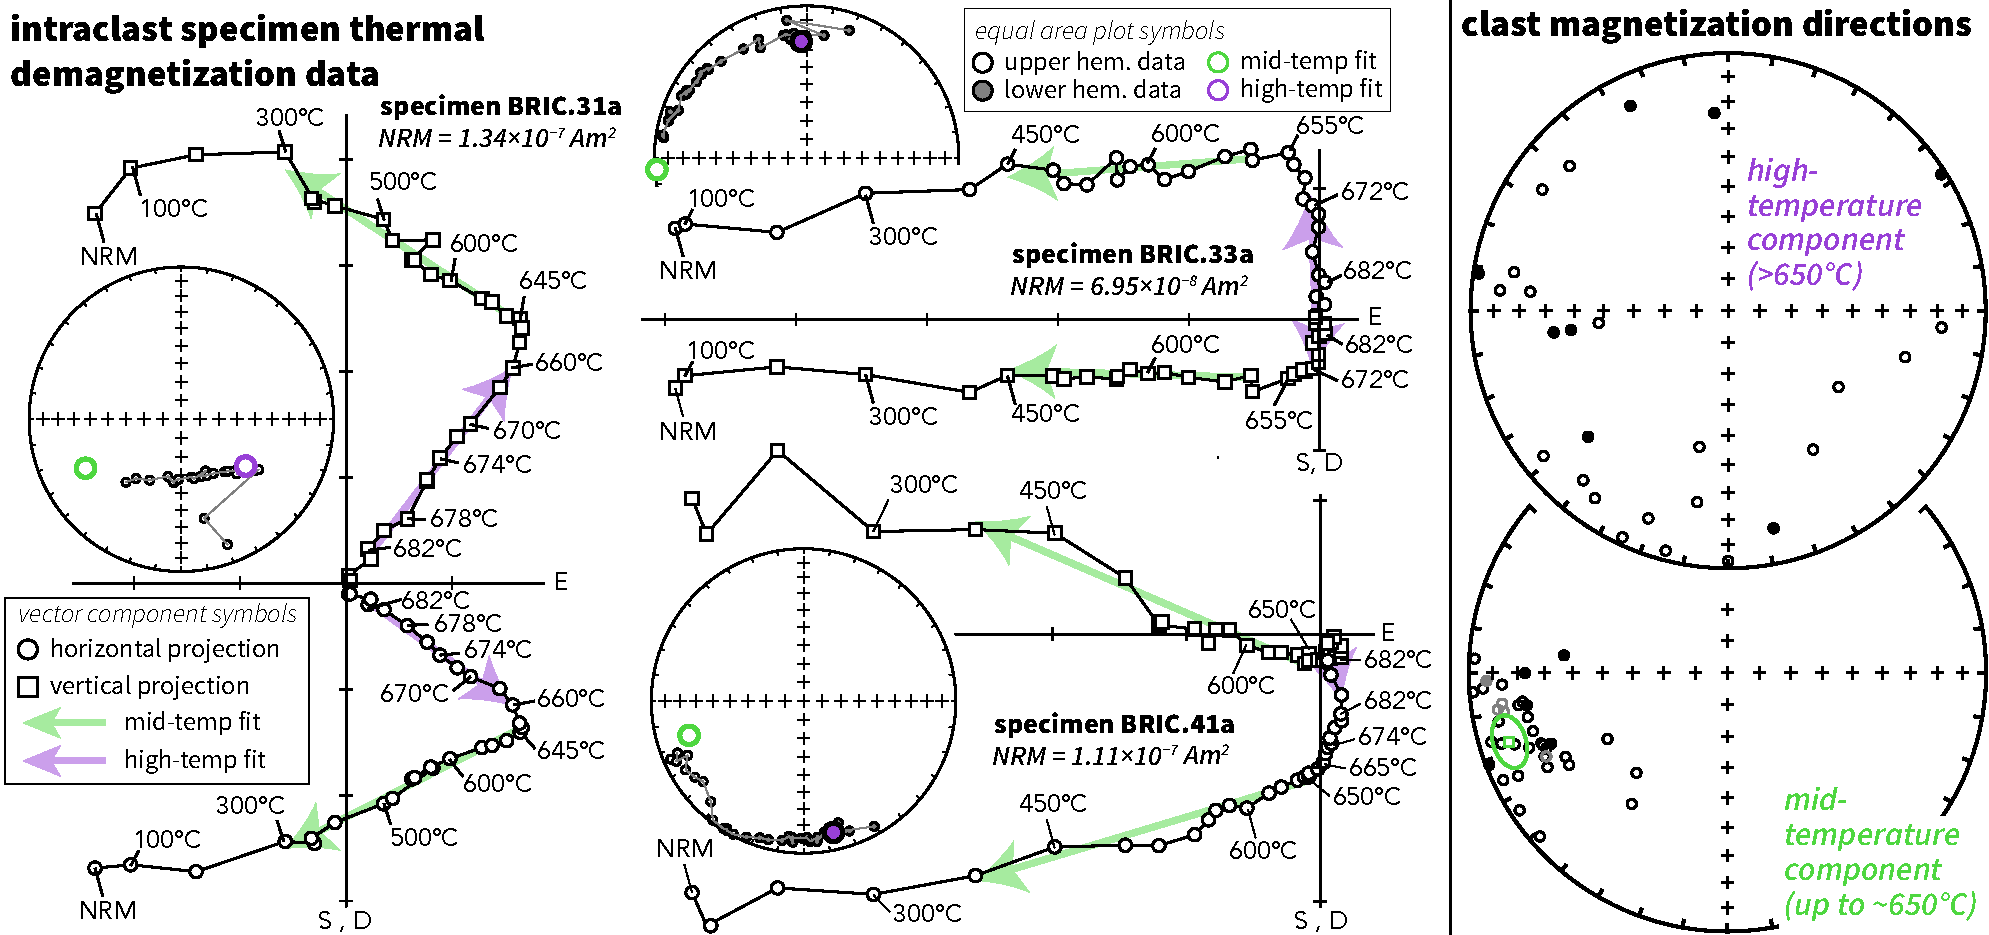
\includegraphics[width=\textwidth]{BRIC_pmag.pdf}
\caption{\small{Paleomagnetic data from intraclasts reveal a mid-temperature component that typically unblocks prior to 655\textdegree C and a high-temperature component that typically unblocks between 655\textdegree C and 687\textdegree C. These components are present as varying fractions of the overall remanence in the three individual clasts for which data are shown on vector component plots and measurement-level equal area plots (developed using PmagPy; \citealp{Tauxe2016a}). The direction of the mid-temperature component is shown as purple arrows on the vector component plots and purple circles on the equal area plots while the high-temperature component is shown with green symbols. The mid-temperature component has a similar direction throughout the clasts as can be seen on the specimen data and the equal area plot that plots the component directions for all samples. In contrast, the high-temperature component directions are dispersed (particularly in declination) indicating that it was acquired very early prior to the siltstone clasts being redeposited within the channel.}}
\label{fig:intraclast_pmag}
\end{figure}

The clasts typically reveal two distinct magnetization directions. One direction was similar throughout the intraclasts and was typically removed from temperatures between 200\textdegree C and 650\textdegree C (Fig. \ref{fig:intraclast_pmag}). The thermal unblocking spectra of this mid-temperature component show a continuous unblocking of magnetic remanence between these temperatures without a ``shoulder'' at $\sim$580\textdegree C that would indicate remanence associated with magnetite. This component is directionally well-grouped indicating that it was acquired following deposition of the clasts (Fig. \ref{fig:intraclast_pmag}). The other component trends towards the origin and is removed by thermal demagnetization steps at the highest levels such that it typically can be fit by a least-square line between 665\textdegree C and 688\textdegree C. The relative magnitude of the components varies between intraclasts (Fig. \ref{fig:intraclast_pmag}). While the high-temperature component can sometimes be fit as a line with a lower temperature bound of 660\textdegree C (BRIC.31a in Fig. \ref{fig:intraclast_pmag}), due to overlapping unblocking temperatures between the mid-temperature and high-temperature components the lower bounds of the high-temperature fits sometimes need to be as high as 680\textdegree C (BRIC.41a in Fig. \ref{fig:intraclast_pmag}). Note that while the Ne\'el temperature of hematite is sometimes given as 675\textdegree C in the paleomagnetic literature, experimental data often shown the Ne\'el temperature to be as high as 690\textdegree C \citep{Ozdemir2006a}. There is typically a significant directional change in the specimen magnetization between the mid-temperature component and the high-temperature component (Fig. \ref{fig:intraclast_pmag}). As a result, 29 of the 39 analyzed intraclast specimens could be fit with distinct mid-temperature and high-temperature least-squares lines. An additional 5 specimens were undergoing directional change through thermal demagnetization indicative of the presence of a distinct high-temperature component, but this component was not well-expressed enough to be fit. 5 of the specimens showed no directional change and could be fit with a single mid-high-temperature component that is grouped with the mid-temperature component. In contrast to the well-grouped mid-temperature component, the high-temperature component directions are dispersed indicating that the component was acquired prior to liberation and redeposition of the clasts. The high-temperature component directions are more dispersed in declination than inclination leading to a distribution that is not randomly dispersed on a sphere. Given that the clasts are tabular and were liberated along their depositional lamination and subsequently landed roughly bedding parallel, it is to be expected that the rotations were largely around a vertical axis preferentially changing declination.

Petrography on the intraclasts reveals two distinct populations of hematite (Fig. \ref{fig:intraclast_images}). One population is fine-grained pigmentary hematite present dominantly within the clay-sized matrix and rimming detrital silt-sized grains. The zones of pigmentary hematite within the matrix remain cloudy to high magnification indicating that the individual grains are submicron in size. The other population of hematite grains has a similar size and shape to other detrital silt-sized grains  -- typically ranging from 2 to 50 $\mu$m in diameter. These hematite grains were identified through reflected light microscopy with their mineralogy supported by energy-dispersive x-ray spectroscopy (EDS) and confirmed by electron backscatter diffraction (EBSD). These mineralogical interpretations, including an overall lack of magnetite, are consistent with those of \cite{Vincenz1968b}. Petrographic work on the underlying Copper Harbor Formation identified hematite grains on the scale of 10s of microns, but concluded that it was ambiguous whether these grains were detrital or authigenic \citep{Elmore1982a}. The dispersion of the paleomagnetic component that is held by such grains in the Freda intraclasts strongly supports that, in the case of the Freda siltstones, these grains were hematite when they were deposited. 

%While $>$1$\mu$m hematite grains within sedimentary rocks can arise through secondary fluid flow and soil formation processes, the directional data strongly support that the interpretation of these larger hematite grains being primary within these lithologies of the Freda Formation.

%Additional Fe-Ti oxides in the intraclasts include rutile, titanite and ilmenite. Some of the hematite grains retain primary exsolution textures consistent with an igneous origin rather than having formed as an authigenic grain insitu.

\section*{DISCUSSION}

Single-domain hematite grains have high coercivities ($>$150 mT; \citealp{Ozdemir2014a}) which combined with their high unblocking temperatures make populations of hematite within rocks stable on long timescales, resistant to overprinting and therefore attractive for paleomagnetic study. In contrast to magnetite, hematite grains retain stable single domain behavior in crystals $>$1$\mu$m with the threshold to multidomain behavior occurring when grain diameters exceed $\sim$100$\mu$m \citep{Kletetschka2002a, Ozdemir2014a}. Hematite nanoparticles with diameters $<$30 nm have superparamagnetic behavior wherein thermal fluctuation energy overwhelms the ability of the grain to retain a stable magnetization at Earth surface temperatures \citep{Ozdemir2014a}. Hematite grains become progressively less influenced by thermal fluctuations as they reach grain sizes of a few hundred nanometers at which point they are stable up to temperatures approaching the N\'eel temperature of $\sim$685\textdegree C \citep{Swanson-Hysell2011a, Ozdemir2014a}. As a result, there is a strong relationship between grain volume and unblocking temperature that can be utilized to estimate grain size. A hematite population that is progressively unblocking at thermal demagnetization steps well below the N\'eel transition temperature, such as the mid-temperature component of the intraclasts, is comprised of grains within the $\sim$30 to $\sim$400 $\mu$m size range. This fine-grain size is consistent with the pigmentary phase within the intraclasts (Fig. \ref{fig:intraclast_images}). 

Given the directional consistency of the mid-temperature component between the intraclasts it must have dominantly formed in the intraclasts after they were redeposited in the channel as a chemical remanent magnetization. Chemical remanent magnetization acquisition by the pigmentary hematite would have occurred as hematite grains grew to sizes above the superparamagnetic to stable single domain transition. In contrast, given its sharp unblocking temperature close to the N\'eel temperature, the high-temperature component is dominantly held by hematite grains that are $>$400$\mu$m such as the silt-sized hematite grains observed petrographically (Fig. \ref{fig:intraclast_images}). That the high-temperature remanence component held by these grains was rotated along with the clasts indicates that it is primary and was acquired prior to the redeposition of the cohesive silt clasts. That this component is held by larger grains sizes supports the interpretation that it is a detrital remanent magnetization rather than a chemical remanent magnetization that formed very early in the sediments prior to clast liberation.

Oxidation of iron in aqueous environments often proceeds through the formation of fine-grained poorly crystalline ferrihydrite which transforms to stable crystalline hematite at neutral pH on geologically short timescales \citep{Cudennec2006a}. The broad unblocking temperatures we observe for the chemical remanent magnetization in the Freda intraclasts is similar to that seen in hematite populations produced through experimental ferrihydrite to hematite conversion \citep{Jiang2015a}. The differential unblocking temperature spectra of the two components within the Freda intraclasts provides strong support for the argument of \cite{Jiang2015a} that chemical remanent magnetization can be distinguished from detrital remanent magnetization on the basis of unblocking temperature spectra with primary detrital remanence unblocking at the highest temperatures approaching the N\'eel temperature. However, it is also clear that while the detrital remanent magnetization can be well isolated at temperatures as low as 650\textdegree C (specimen BRIC.31a in Fig. \ref{fig:intraclast_pmag}) that the chemical remanent magnetization thermal unblocking spectra can overlap with that of the detrital remanence and extend up to temperatures closer to the N\'eel temperature (specimen BRIC.41a in Fig. \ref{fig:intraclast_pmag}). Therefore, to isolate primary remanence in red beds, best practice should be to proceed with very high-resolution thermal demagnetization steps above 600\textdegree C, and particularly above 650\textdegree C. These intraclast data reveal that directional change at the highest unblocking temperatures provides an effective means to discriminate primary and secondary magnetizations within siltstones of the Freda formation and other red beds. 

%This discrimination is an approach taken among practitioners with the characteristic remanent magnetization for a sample typically being defined as the component removed at the uppermost steps of thermal demagnetization \cite{Van-Der-Voo2012a}. This practice gains additional credibility with these results. 

%The clay-component of the sediment that provided the cohesion to the clasts when they were eroded could, by lowering the permeability, have prevent ox 
 
%\subsection*{CONCLUSIONS}
%
%Sedimentary rocks containing hematite form very important records of paleomagnetic data through time that bear on interpretations of patterns of geomagnetic reversals and the past position of continents. However, hematite can form as a product of mineral transformations in the near-surface environment. As a result, it can be difficult to constrain the timing of hematite formation. The paleomagnetic results on the Freda Formation intraclasts, combined with their depositional context, reveal that the siltstones record both a primary direction held by detrital grains and a secondary direction held by pigmentary hematite. These demonstrably primary and secondary components can be differentiated by their differential thermal unblocking spectra. Very high-resolution thermal demagnetization that seeks to 

\subsection*{ACKNOWLEDGEMENTS}
\footnotesize

This research was supported by the Esper S. Larsen, Jr. Research Fund and the National Science Foundation through grant EAR-1419894. SPS was supported by the Miller Institute for Basic Research in Science. The Wisconsin Department of Natural Resources granted a research and collection permit that enabled sampling within Copper Falls State Park. Oliver Abbitt assisted with field work and Taiyi Yang assisted with paleomagnetic analyses. 

\singlespacing

\newpage

\bibliographystyle{gsabull}
\bibliography{../../references/allrefs}

\end{document}